\subsection{Age (8)}
    \begin{align*}
      \text{PrehistoricAge} \to& \text{Age}\\
      \text{Antiquity} \to& \text{[AND}\\
      &\quad\text{Age}\\
      &\quad\text{[FILLS :succeededBy MiddleAges]]}\\\\
      \text{MiddleAges} \to& \text{[AND}\\
      &\quad\text{Age}\\
      &\quad\text{[FILLS :precededBy Antiquity]}\\
      &\quad\text{[FILLS :succeededBy Renaissance]]}\\\\  
      \text{GothicAge} \to& \text{[AND}\\
      &\quad\text{Age}\\
      &\quad\text{[FILLS :precededBy MiddleAges]}\\
      &\quad\text{[FILLS :succeededBy Renaissance]]}\\\\
      \text{Renaissance} \to& \text{[AND}\\
      &\quad\text{Age}\\
      &\quad\text{[FILLS :precededBy MiddleAges]}\\
      &\quad\text{[FILLS :succeededBy NewAge]]}\\\\
      \text{NewAge} \to& \text{[AND}\\
      &\quad\text{Age}\\
      &\quad\text{[FILLS :precededBy Renaissance]}\\
      &\quad\text{[FILLS :succeededBy ModernAge]]}\\\\
      \text{ModernAge} \to& \text{[AND}\\
      &\quad\text{Age}\\
      &\quad\text{[FILLS :precededBy NewAge]}\\
      &\quad\text{[FILLS :succeededBy ContemporaryAge]]}\\\\
      \text{ContemporaryAge} \to& \text{[AND}\\
      &\quad\text{Age}\\
      &\quad\text{[FILLS :precededBy ModernAge]]}
    \end{align*}
    
  \subsection{Style (25)}
    \begin{align*}
      \text{Paleolithic} \to& \text{[AND}\\
      &\quad\text{Style}\\
      &\quad\text{[FILLS :belongsTo PrehistoricAge]]}\\\\
      \text{Neolithic} \to& \text{[AND}\\
      &\quad\text{Style}\\
      &\quad\text{[FILLS :belongsTo PrehistoricAge]]}\\\\
      \text{AncientEgyptian} \to& \text{[AND}\\
      &\quad\text{Style}\\
      &\quad\text{[FILLS :belongsTo Antiquity]]}\\\\
      \text{AncientGreek} \to& \text{[AND}\\
      &\quad\text{Style}\\
      &\quad\text{[FILLS :belongsTo Antiquity]}\\
      &\quad\text{[FILLS :positiveReactionTo AncientEgyptian]]}\\\\
      \text{Roman} \to& \text{[AND}\\
      &\quad\text{Style}\\
      &\quad\text{[FILLS :belongsTo Antiquity]}\\
      &\quad\text{[FILLS :positiveReactionTo AncientGreek]]}\\\\
      \text{Byzantine} \to& \text{[AND}\\
      &\quad\text{Style}\\
      &\quad\text{[FILLS :belongsTo MiddleAges]]}\\\\
      \text{Romanesque} \to& \text{[AND}\\
      &\quad\text{Style}\\
      &\quad\text{[FILLS :belongsTo MiddleAges]]}\\\\
      \text{Gothic} \to& \text{[AND}\\
      &\quad\text{Style}\\
      &\quad\text{[FILLS :belongsTo GothicAge]}\\
      &\quad\text{[FILLS :positiveReactionTo Romanesque]]}\\\\
      \text{ItalianRenaissance} \to& \text{[AND}\\
      &\quad\text{Style}\\
      &\quad\text{[FILLS :belongsTo Renaissance]}\\
      &\quad\text{[FILLS :negativeReactionTo Gothic]]}\\\\
      \text{NordicRenaissance} \to& \text{[AND}\\
      &\quad\text{Style}\\
      &\quad\text{[FILLS :belongsTo Renaissance]]}\\\\
      \text{Baroque} \to& \text{[AND}\\
      &\quad\text{Style}\\
      &\quad\text{[FILLS :belongsTo NewAge]}\\
      &\quad\text{[FILLS :negativeReactionTo Renaissance]]}\\\\
      \text{Rococo} \to& \text{[AND}\\
      &\quad\text{Style}\\
      &\quad\text{[FILLS :belongsTo NewAge]}\\
      &\quad\text{[FILLS :negativeReactionTo Baroque]]}\\\\
      \text{Classicism} \to& \text{[AND}\\
      &\quad\text{Style}\\
      &\quad\text{[FILLS :belongsTo NewAge]}\\
      &\quad\text{[FILLS :negativeReactionTo Rococo]]}\\\\
      \text{Romanticism} \to& \text{[AND}\\
      &\quad\text{Style}\\
      &\quad\text{[FILLS :belongsTo NewAge]]}\\\\
      \text{Realism} \to& \text{[AND}\\
      &\quad\text{Style}\\
      &\quad\text{[FILLS :belongsTo ModernAge]}\\
      &\quad\text{[FILLS :negativeReactionTo Romanticism]]}\\\\
      \text{Impressionism} \to& \text{[AND}\\
      &\quad\text{Style}\\
      &\quad\text{[FILLS :belongsTo ModernAge]}\\
      &\quad\text{[FILLS :negativeReactionTo Realism]]}\\\\
      \text{PostImpressionism} \to& \text{[AND}\\
      &\quad\text{Style}\\
      &\quad\text{[FILLS :belongsTo ModernAge]}\\
      &\quad\text{[FILLS :positiveReactionTo Impressionism]]}\\\\
      \text{Expressionism} \to& \text{[AND}\\
      &\quad\text{Style}\\
      &\quad\text{[FILLS :belongsTo ModernAge]}\\
      &\quad\text{[FILLS :negativeReactionTo Realism]]}\\\\
      \text{Cubism} \to& \text{[AND}\\
      &\quad\text{Style}\\
      &\quad\text{[FILLS :belongsTo ModernAge]}\\
      &\quad\text{[FILLS :negativeReactionTo Impressionism]]}\\\\
      \text{Futurism} \to& \text{[AND}\\
      &\quad\text{Style}\\
      &\quad\text{[FILLS :belongsTo ModernAge]]}\\\\
      \text{Dadaism} \to& \text{[AND}\\
      &\quad\text{Style}\\
      &\quad\text{[FILLS :belongsTo ModernAge]]}\\\\
      \text{Surrealism} \to& \text{[AND}\\
      &\quad\text{Style}\\
      &\quad\text{[FILLS :belongsTo ModernAge]}\\
      &\quad\text{[FILLS :positiveReactionTo Dadaism]]}\\\\
      \text{PopArt} \to& \text{[AND}\\
      &\quad\text{Style}\\
      &\quad\text{[FILLS :belongsTo ContemporaryAge]]}\\\\
      \text{ConceptualArt} \to& \text{[AND}\\
      &\quad\text{Style}\\
      &\quad\text{[FILLS :belongsTo ContemporaryAge]}\\
      &\quad\text{[FILLS :positiveReactionTo PopArt]]}
    \end{align*}
    \subsection{Region (7)}
        \begin{align*}
        \text{Asia} &\to \text{Region}\\
        \text{Africa} &\to \text{Region}\\
        \text{Australia} &\to \text{Region}\\
        \text{SouthAmerica} &\to \text{Region}\\
        \text{NorthAmerica} &\to \text{Region}\\
        \text{EasternEurope} &\to \text{Region}\\
        \text{WesternEurope} &\to \text{Region}
        \end{align*}
    \subsection{Medium (4)}
        \begin{align*}
        \text{Chalk} &\to \text{Medium}\\
        \text{Graphite} &\to \text{Medium}\\
        \text{OilPaint} &\to \text{Paint} \sqsubseteq \text{Medium}\\
        \text{AcrylicPaint} &\to \text{Paint} \sqsubseteq \text{Medium}
        \end{align*}
    \subsection{Depiction (6)}
        \begin{align*}
        \text{AbstractDepiction} &\to \text{Depiction}\\
        \text{GroupScene} &\to \text{Depiction}\\
        \text{Portrait} &\to \text{Depiction}\\
        \text{HistoricalEvent} &\to \text{Depiction}\\
        \text{UrbanLandscape} &\to \text{Landscape}\sqsubseteq \text{Depiction}\\
        \text{NaturalLandscape} &\to \text{Landscape}\sqsubseteq \text{Depiction}\\
        \end{align*}
    \subsection{Artist (7)}
    \begin{align*}
    \text{Michelangelo} \to& \text{[AND} \\
    &\quad \text{Artist} \\
    &\quad \text{[FILLS :livedIn WesternEurope]]} \\
    \text{VincentVanGogh} \to& \text{[AND} \\
    &\quad \text{Artist} \\
    &\quad \text{[FILLS :livedIn WesternEurope]]} \\
    \text{JohannesVermeer} \to& \text{[AND} \\
    &\quad \text{Artist} \\
    &\quad \text{[FILLS :livedIn WesternEurope]]} \\
    \text{LeonardoDaVinci} \to& \text{[AND} \\
    &\quad \text{Artist} \\
    &\quad \text{[FILLS :livedIn WesternEurope]]} \\
    \text{FranciscoGoya} \to& \text{[AND} \\
    &\quad \text{Artist} \\
    &\quad \text{[FILLS :livedIn WesternEurope]]} \\
    \text{AndyWarhol} \to& \text{[AND} \\
    &\quad \text{Artist} \\
    &\quad \text{[FILLS :livedIn NorthAmerica]]} \\
    \text{ClaudeMonet} \to& \text{[AND} \\
    &\quad \text{Artist} \\
    &\quad \text{[FILLS :livedIn WesternEurope]]}
    \end{align*}
    
    \subsection{Museum (7)}
    \begin{align*}
    \text{GalleriaDellAccademia} \to& \text{[AND} \\
    &\quad \text{Museum} \\
    &\quad \text{[FILLS :locatedIn WesternEurope]]} \\
    \text{LouvreMuseum} \to& \text{[AND} \\
    &\quad \text{Museum} \\
    &\quad \text{[FILLS :locatedIn WesternEurope]]} \\
    \text{MoMA} \to& \text{[AND} \\
    &\quad \text{Museum} \\
    &\quad \text{[FILLS :locatedIn NorthAmerica]]} \\
    \text{PradoMuseum} \to& \text{[AND} \\
    &\quad \text{Museum} \\
    &\quad \text{[FILLS :locatedIn WesternEurope]]} \\
    \text{KatheKollwitzMuseum} \to& \text{[AND} \\
    &\quad \text{Museum} \\
    &\quad \text{[FILLS :locatedIn WesternEurope]]} \\
    \text{BibliotecaRealeTurin} \to& \text{[AND} \\
    &\quad \text{Museum} \\
    &\quad \text{[FILLS :locatedIn WesternEurope]]} \\
    \text{Mauritshuis} \to& \text{[AND} \\
    &\quad \text{Museum} \\
    &\quad \text{[FILLS :locatedIn WesternEurope]]}
    \end{align*}
    
    \subsection{Artwork (1)}
    Произведения на изкуството, които не са картини.
    \begin{align*}
      \text{David} \to& \text{[AND}\\
      &\quad\text{Artwork}\\
      &\quad\text{[FILLS :createdBy Michelangelo]}\\
      &\quad\text{[FILLS :represents ItalianRenaissance]}\\
      &\quad\text{[FILLS :housedIn GalleriaDellAccademia]]}
    \end{align*}
    \subsection{Painting (7)}
    \begin{itemize}
      \item \textbf{MonaLisa}
        \begin{align*}
          \text{MonaLisa} \to& \text{[AND PortraitPainting, PortraitOilPainting}\\
          &\quad\text{[FILLS :createdBy LeonardoDaVinci]}\\
          &\quad\text{[FILLS :depicts Portrait]}\\
          &\quad\text{[FILLS :usesMedium OilPaint]}\\
          &\quad\text{[FILLS :represents ItalianRenaissance]}\\
          &\quad\text{[FILLS :housedIn LouvreMuseum]]}
        \end{align*}
        \begin{figure}[H]
          \centering
          \includegraphics[width=0.25\linewidth]{images/monalisa.jpg}
        \end{figure}
      \pagebreak
      \item \textbf{PortraitOfAManInRedChalk}
        \begin{align*}
          \text{PortraitOfAManInRedChalk} \to& \text{[AND PortraitPainting}\\
          &\quad\text{[FILLS :createdBy LeonardoDaVinci]}\\
          &\quad\text{[FILLS :depicts Portrait]}\\
          &\quad\text{[FILLS :usesMedium Chalk]}\\
          &\quad\text{[FILLS :represents ItalianRenaissance]}\\
          &\quad\text{[FILLS :housedIn BibliotecaRealeTurin]]}
        \end{align*}
        \begin{figure}[H]
          \centering
          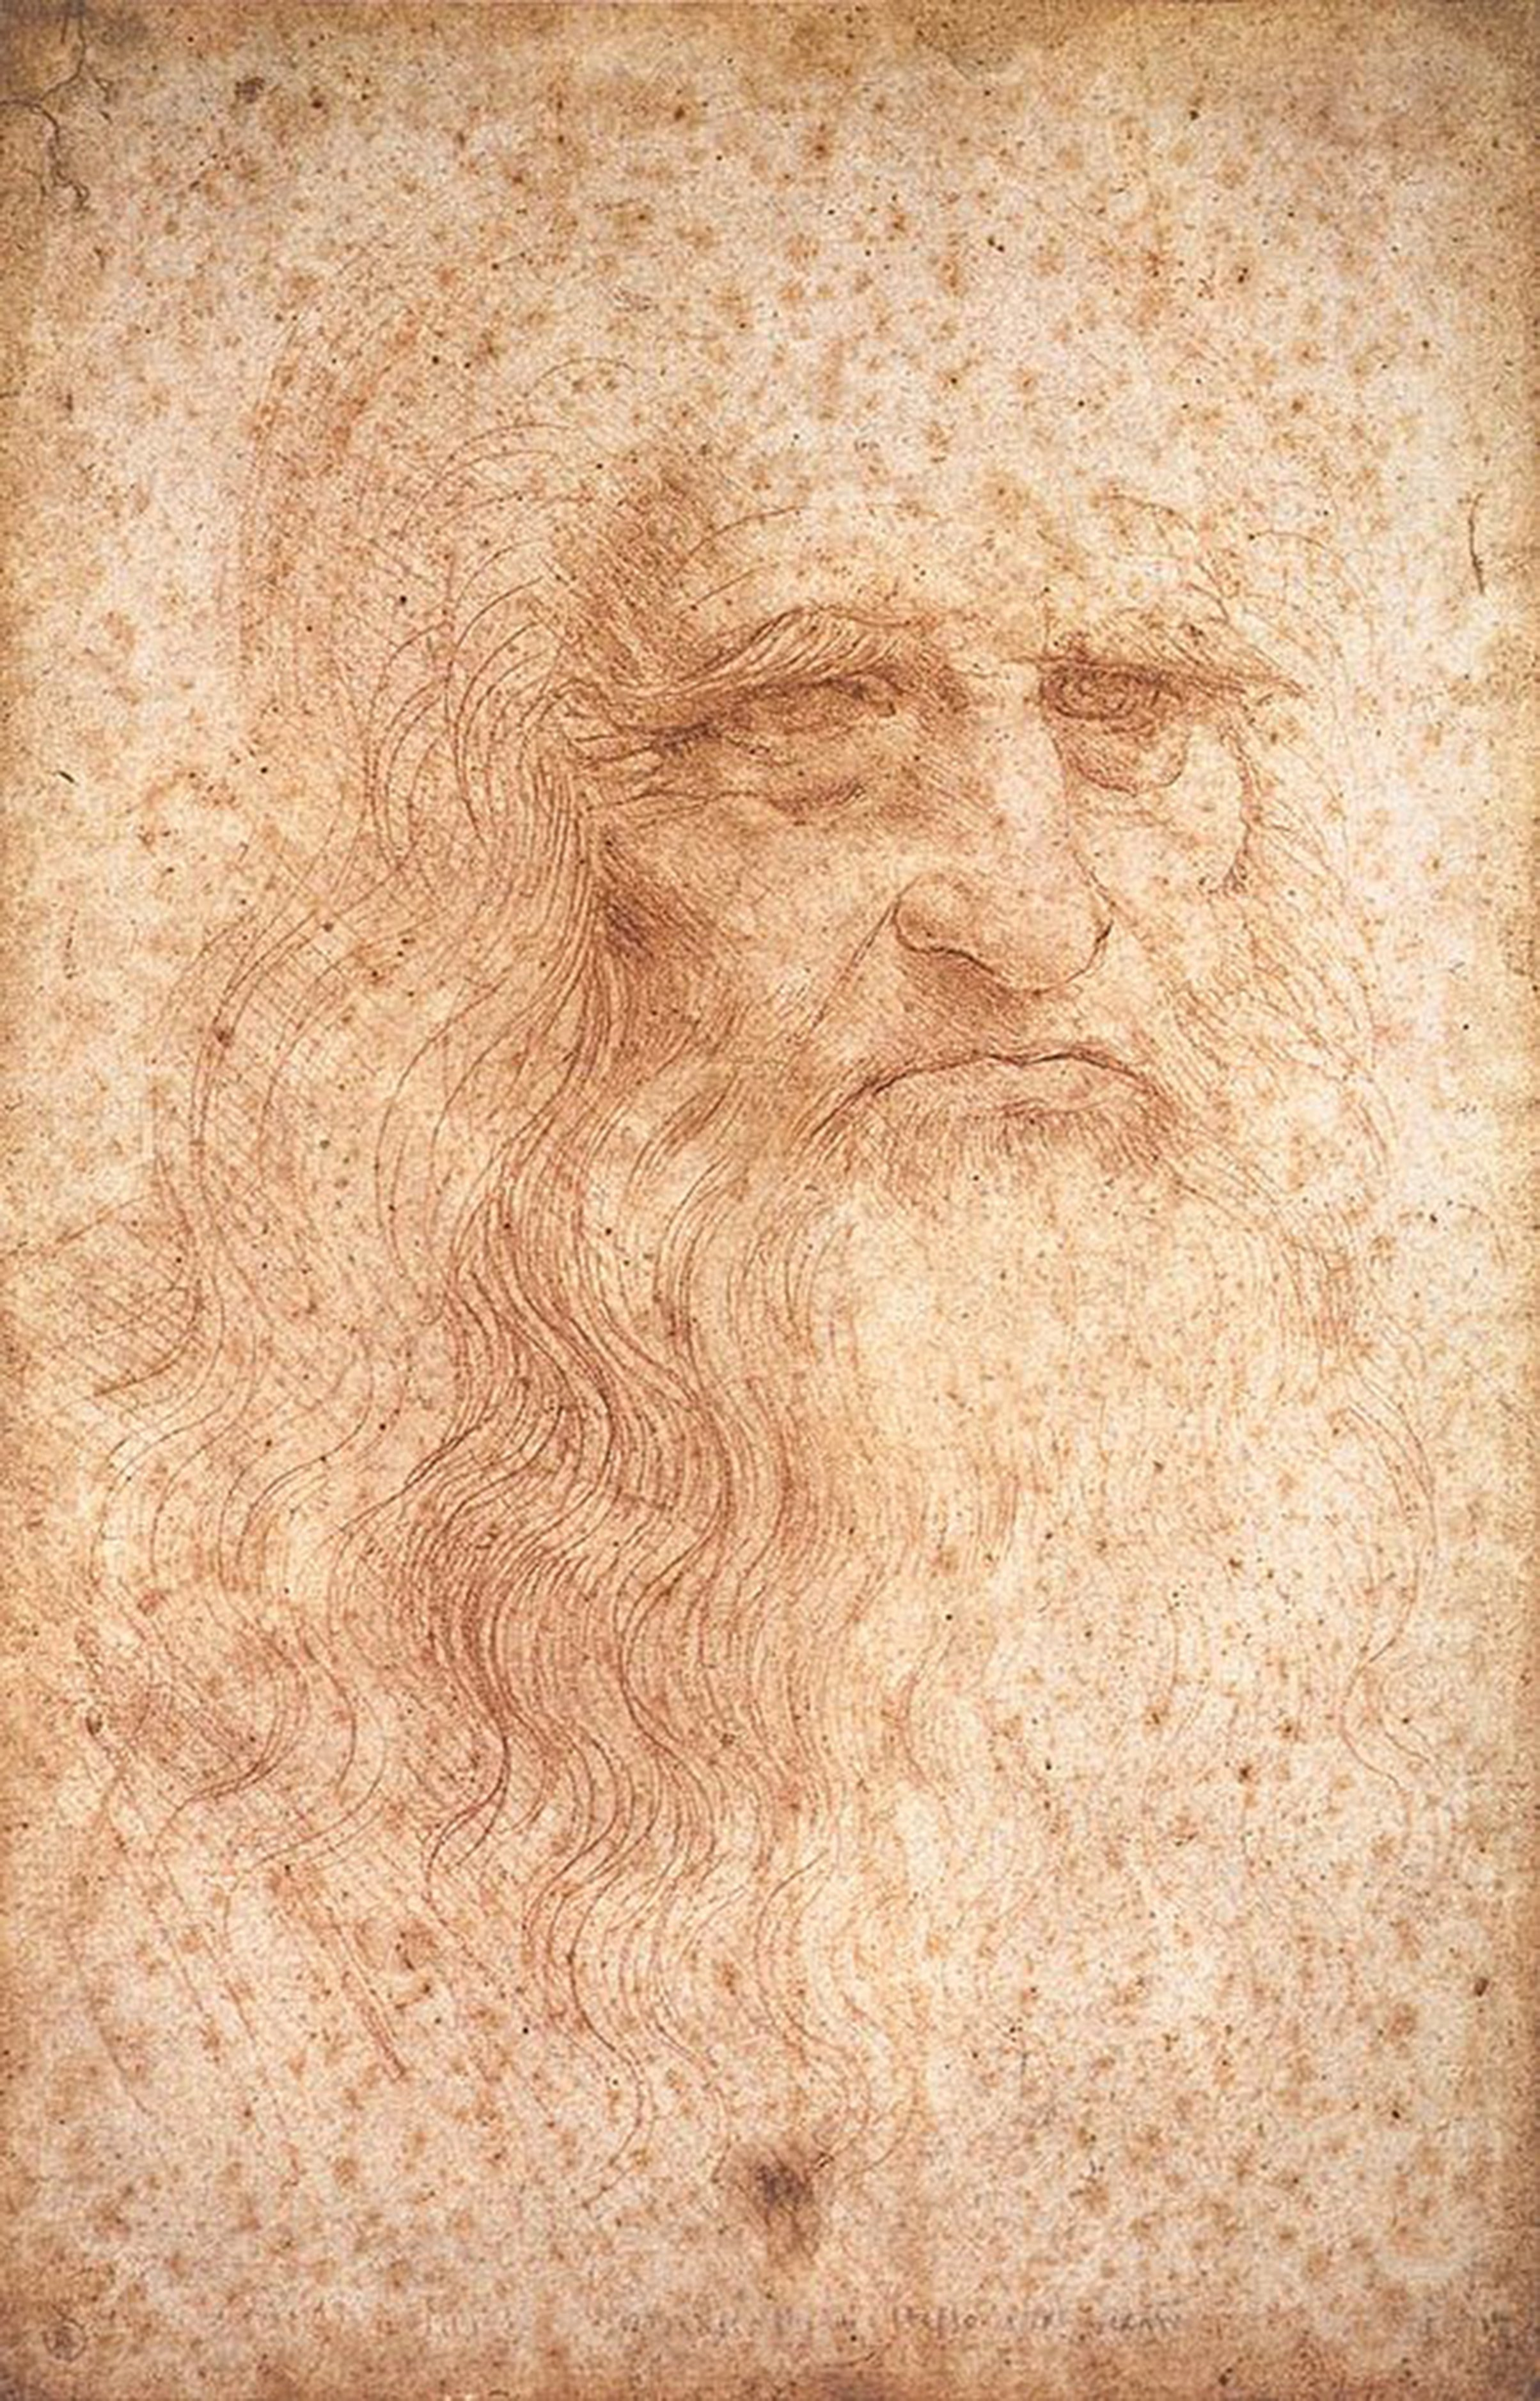
\includegraphics[width=0.35\linewidth]{images/maninredchalk.jpg}
        \end{figure}
      \pagebreak
      \item \textbf{GirlWithAPearlEarring}
        \begin{align*}
          \text{GirlWithAPearlEarring} \to& \text{[AND PortraitPainting, PortraitOilPainting}\\
          &\quad\text{[FILLS :createdBy JohannesVermeer]}\\
          &\quad\text{[FILLS :depicts Portrait]}\\
          &\quad\text{[FILLS :usesMedium OilPaint]}\\
          &\quad\text{[FILLS :represents Baroque]}\\
          &\quad\text{[FILLS :housedIn Mauritshuis]]}
        \end{align*}
        \begin{figure}[H]
          \centering
          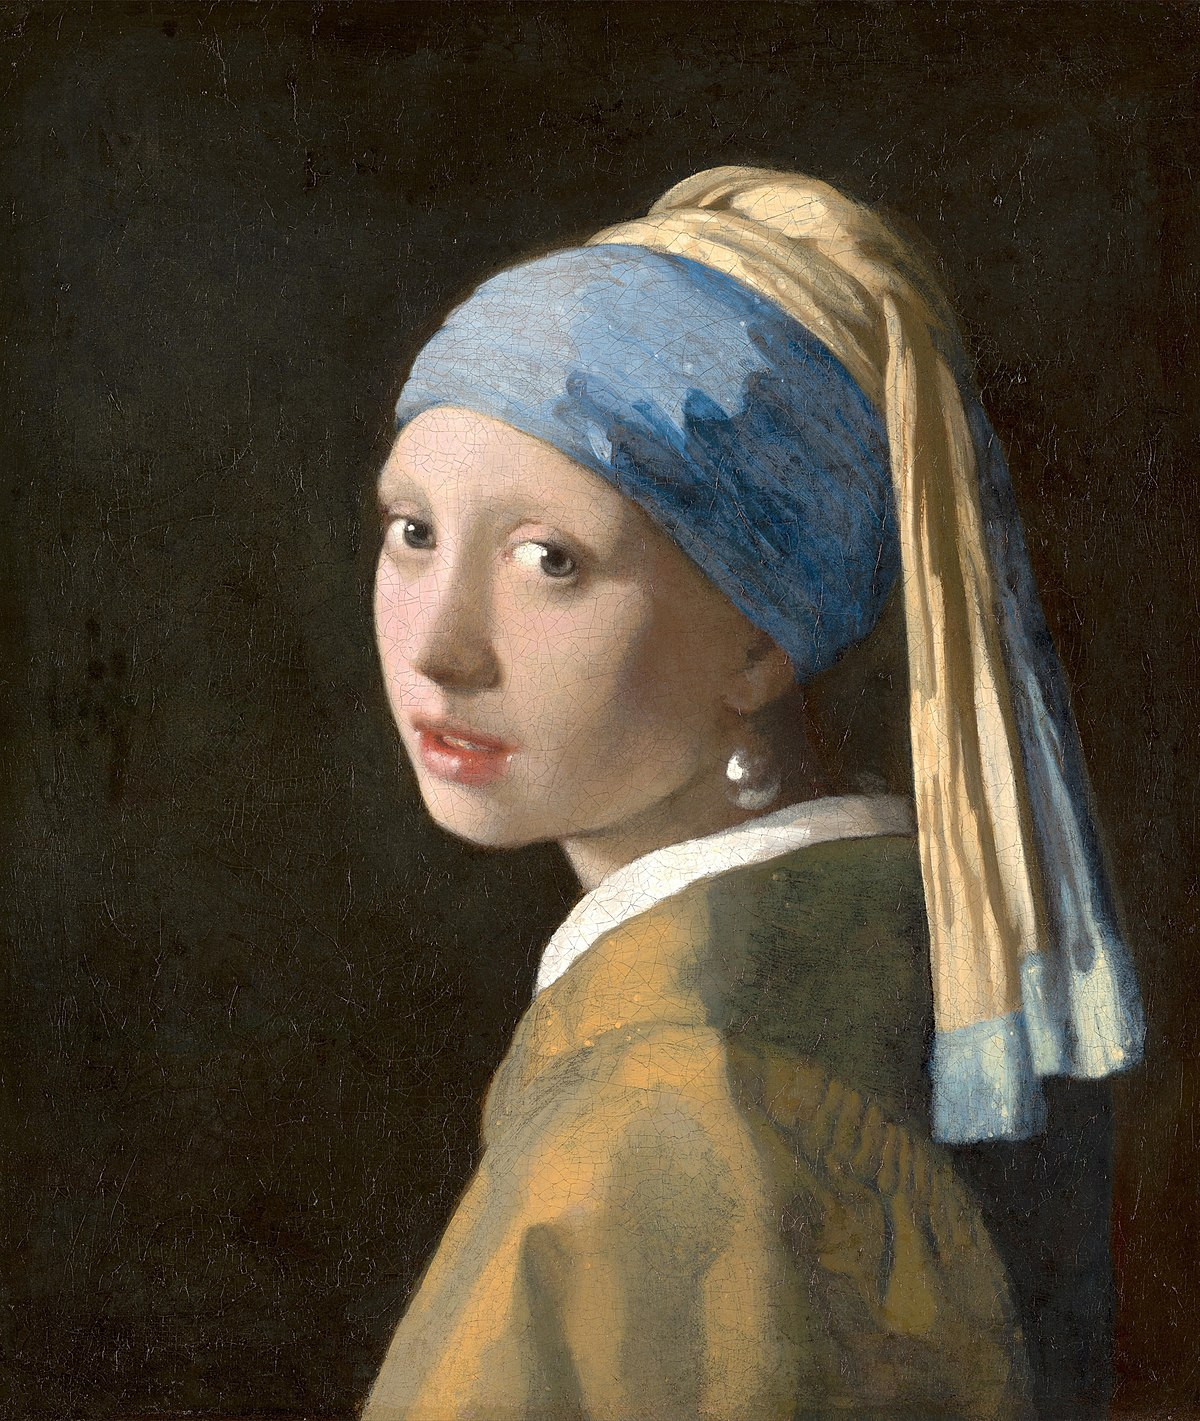
\includegraphics[width=0.35\linewidth]{images/girlwithpearlearring.jpg}
        \end{figure}
      \pagebreak
      \item \textbf{CampbellsSoupCans}
        \begin{align*}
          \text{CampbellsSoupCans} \to& \text{[AND AcrylicPainting}\\
          &\quad\text{[FILLS :createdBy AndyWarhol]}\\
          &\quad\text{[FILLS :depicts AbstractDepiction]}\\
          &\quad\text{[FILLS :usesMedium AcrylicPaint]}\\
          &\quad\text{[FILLS :represents PopArt]}\\
          &\quad\text{[FILLS :housedIn MoMA]]}
        \end{align*}
        \begin{figure}[H]
          \centering
          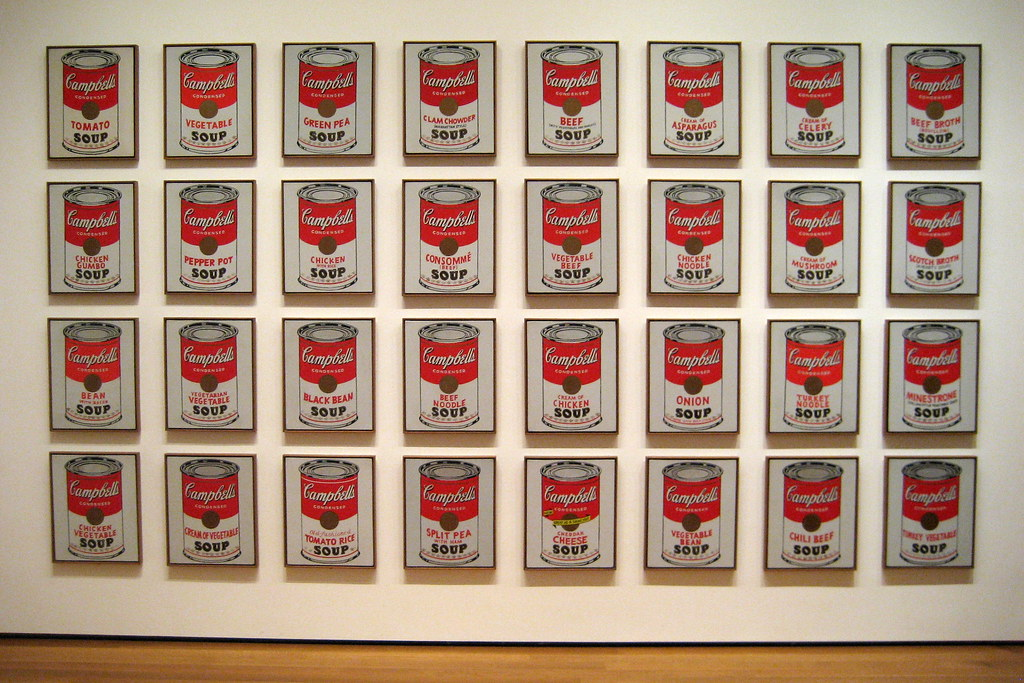
\includegraphics[width=\linewidth]{images/campbellcans.jpg}
        \end{figure}
      \pagebreak
      \item \textbf{ThirdOfMay1808}
        \begin{align*}
          \text{ThirdOfMay1808} \to& \text{[AND HistoricalEventOilPainting}\\
          &\quad\text{[FILLS :createdBy FranciscoGoya]}\\
          &\quad\text{[FILLS :depicts HistoricalEvent]}\\
          &\quad\text{[FILLS :usesMedium OilPaint]}\\
          &\quad\text{[FILLS :represents Romanticism]}\\
          &\quad\text{[FILLS :housedIn PradoMuseum]]}
        \end{align*}
        \begin{figure}[H]
          \centering
          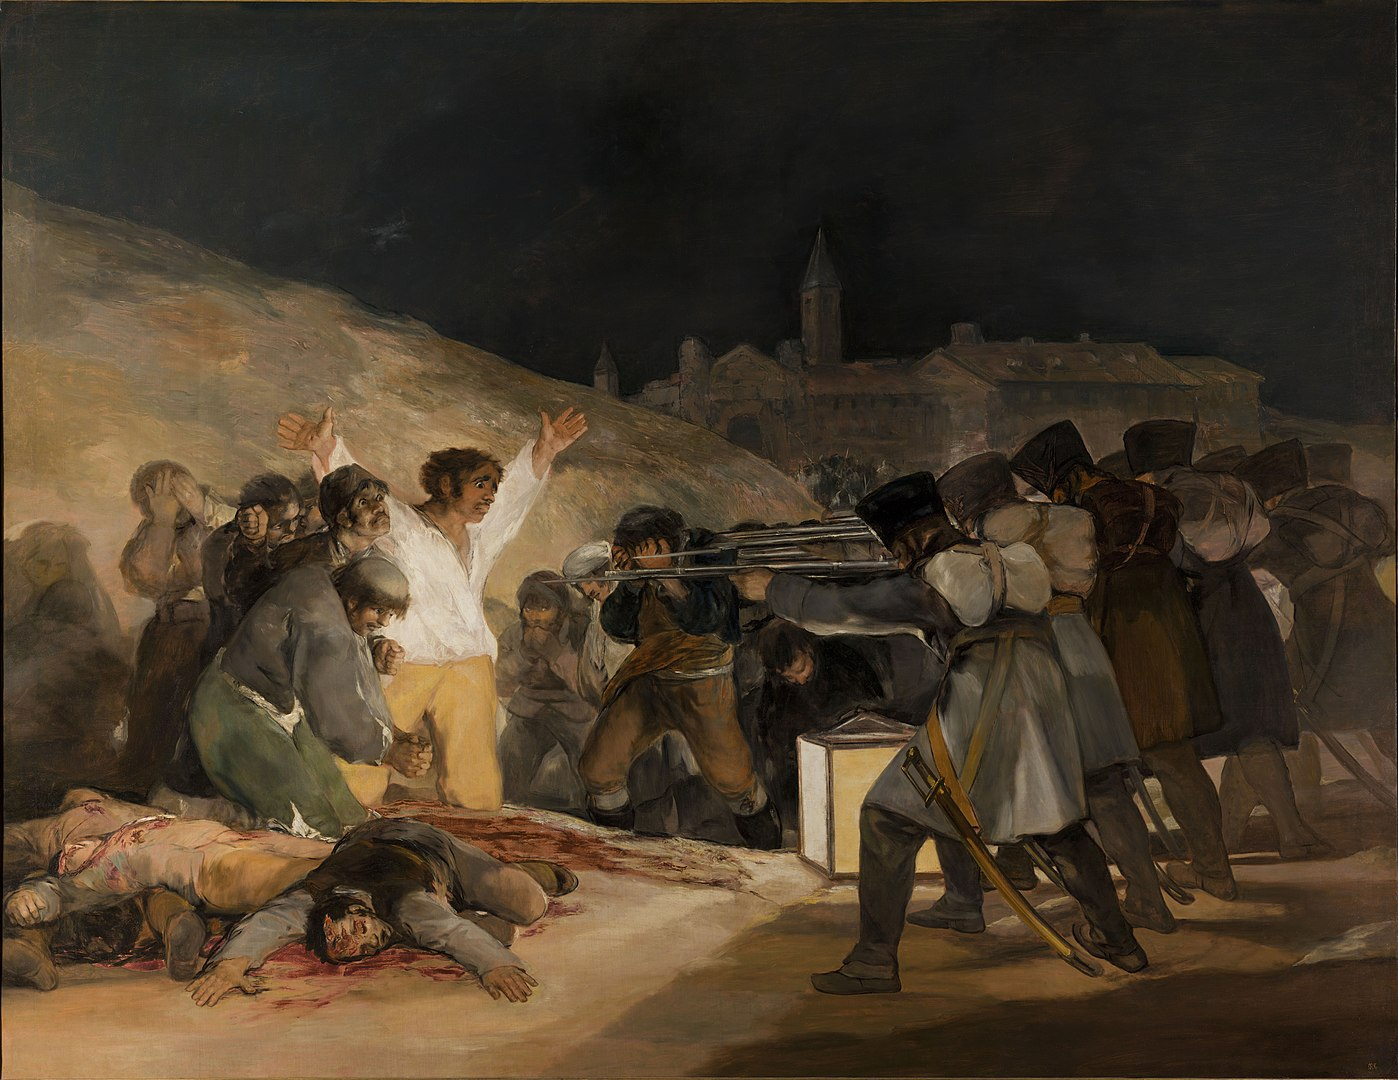
\includegraphics[width=\linewidth]{images/thirdofmay.jpg}
        \end{figure}
      \pagebreak
      \item \textbf{Haystacks}
        \begin{align*}
          \text{Haystacks} \to& \text{[AND LandscapePainting}\\
          &\quad\text{[FILLS :createdBy ClaudeMonet]}\\
          &\quad\text{[FILLS :depicts NaturalLandscape]}\\
          &\quad\text{[FILLS :usesMedium OilPaint]}\\
          &\quad\text{[FILLS :represents Impressionism]}\\
          &\quad\text{[FILLS :housedIn ArtInstituteOfChicago]]}
        \end{align*}
        \begin{figure}[H]
          \centering
          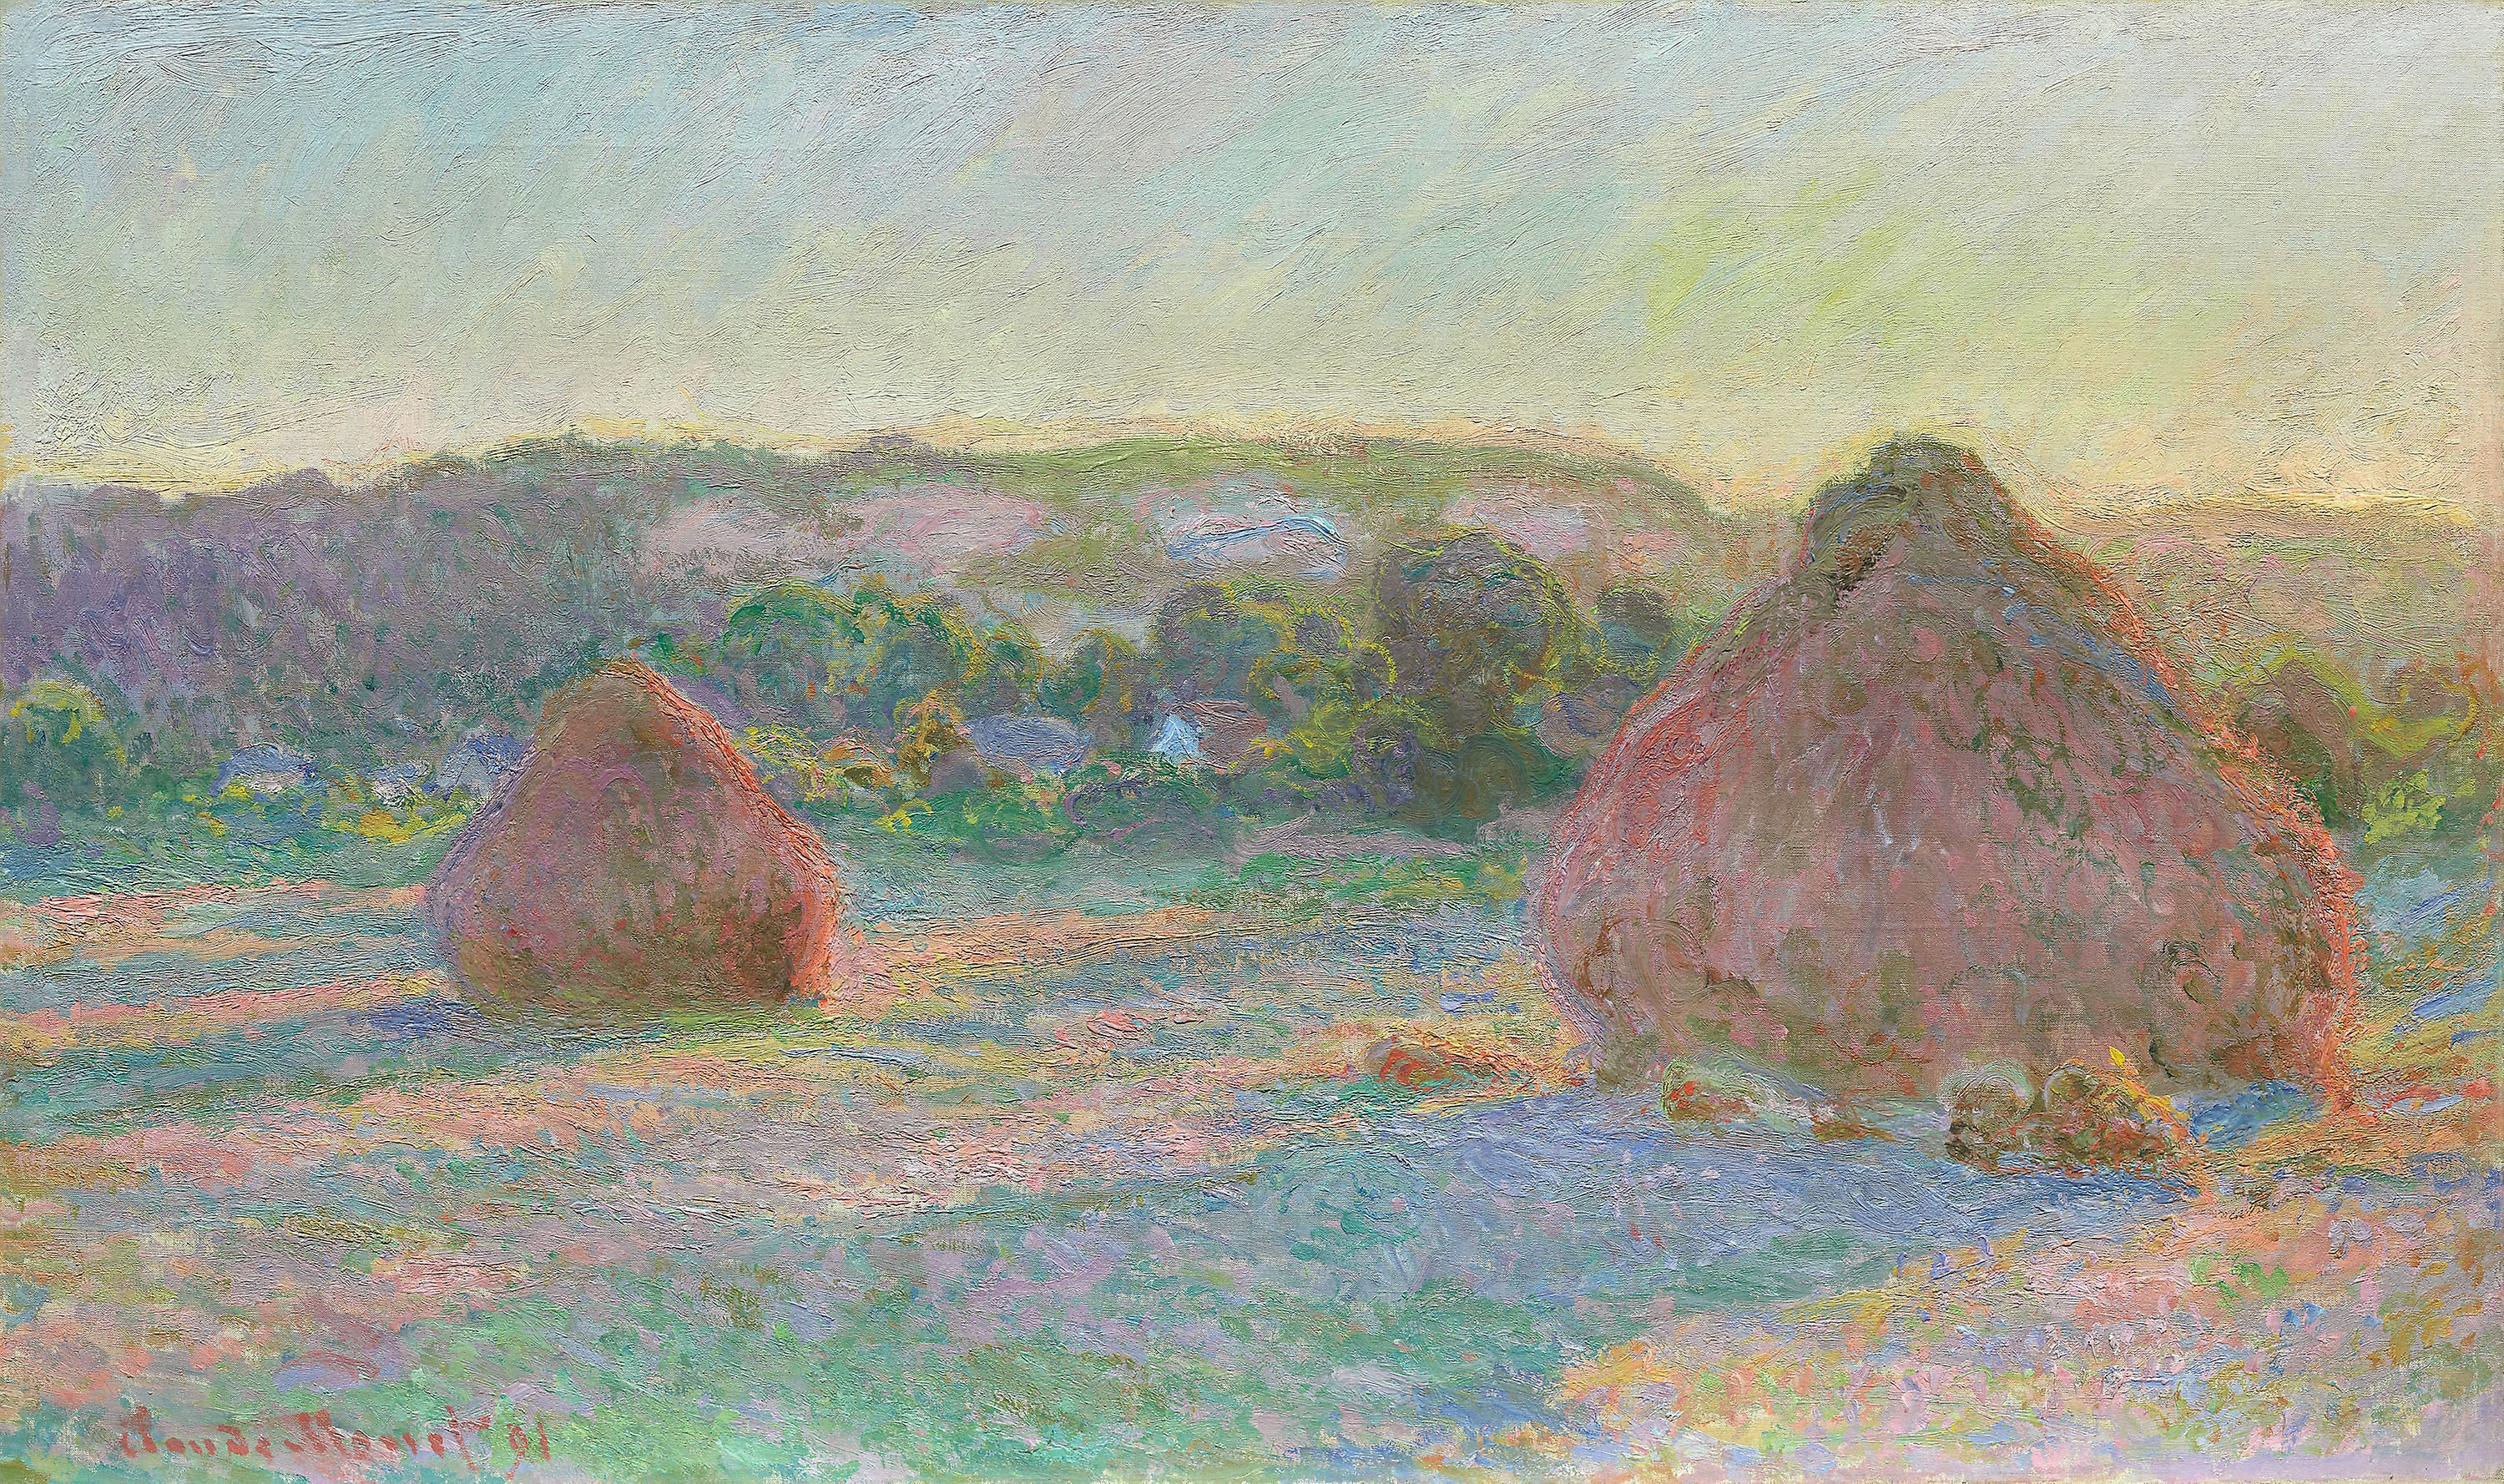
\includegraphics[width=\linewidth]{images/haystacks.jpg}
        \end{figure}
      \pagebreak
      \item \textbf{StarryNightOverTheRhone}
        \begin{align*}
          \text{StarryNightOverTheRhone} \to& \text{[AND LandscapePainting}\\
          &\quad\text{[FILLS :createdBy VincentVanGogh]}\\
          &\quad\text{[FILLS :depicts NaturalLandscape]}\\
          &\quad\text{[FILLS :usesMedium OilPaint]}\\
          &\quad\text{[FILLS :represents PostImpressionism]}\\
          &\quad\text{[FILLS :housedIn MoMA]]}
        \end{align*}
        \begin{figure}[H]
          \centering
          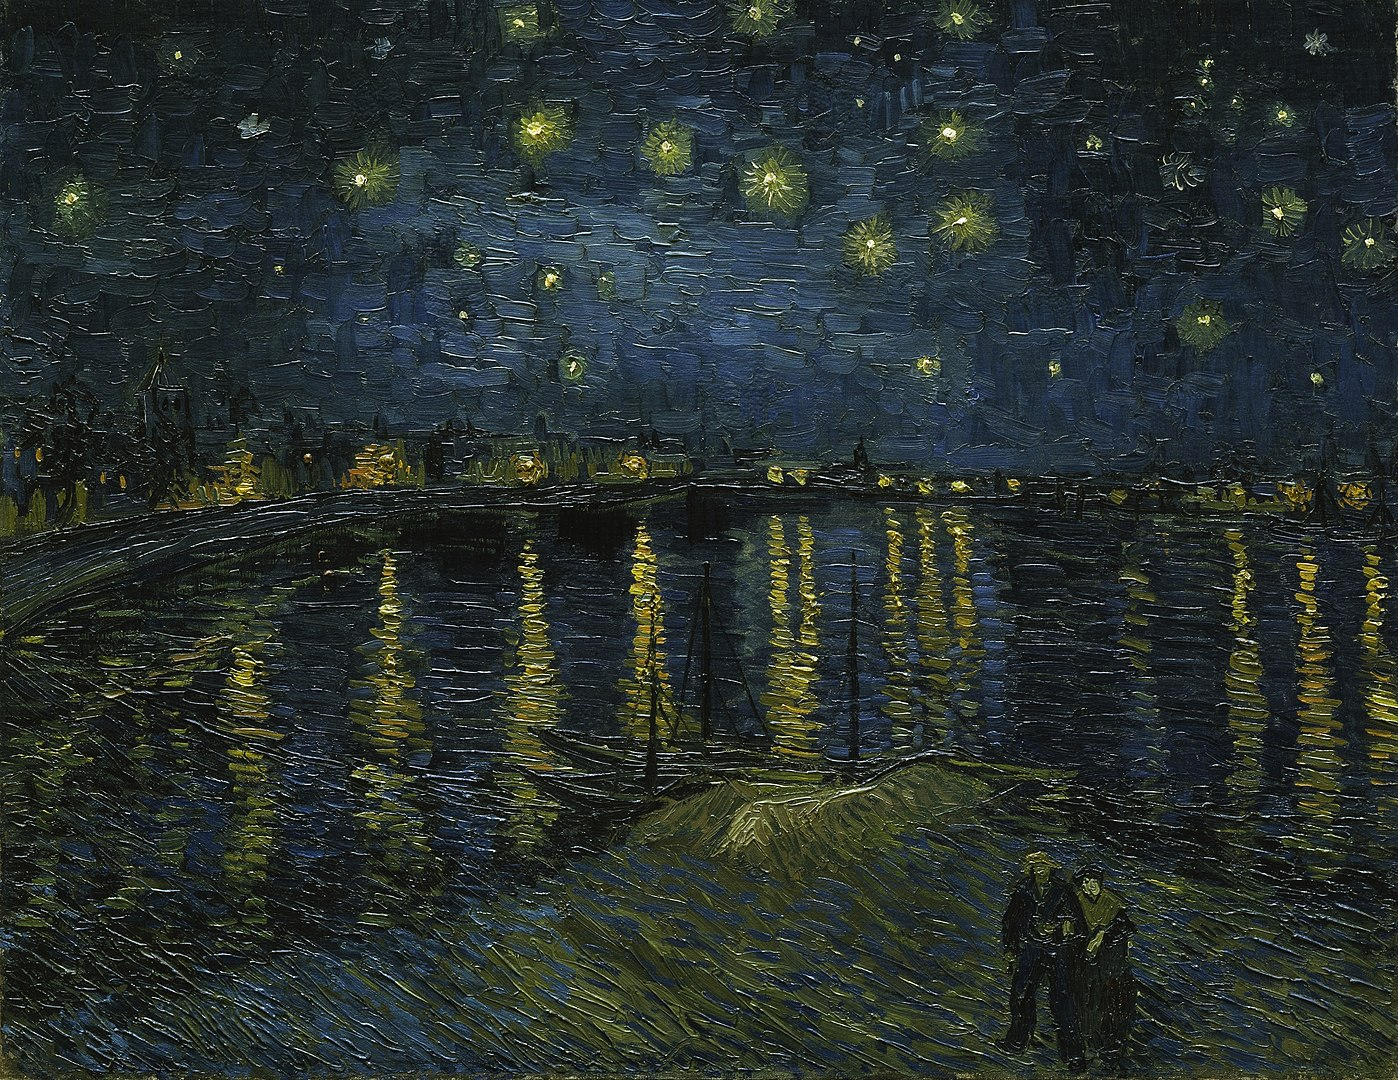
\includegraphics[width=\linewidth]{images/starrynightovertherhone.jpg}
        \end{figure}
    \end{itemize}